\section{\texttt{Introduction}}
\begin{frame}{\textbf{Motivation}}
\begin{figure}
	\centering
	\begin{subfigure}[c]{0.4\textwidth}
		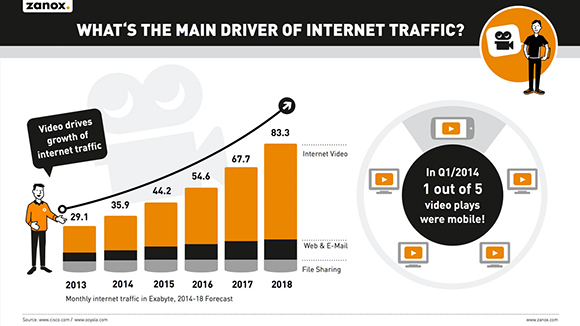
\includegraphics[width=\textwidth]{./img/motivation0.png} 
		 \begin{scriptsize} \begin{center}
		 \textbf{Bloat in Video content \footnotemark}
		\end{center} \end{scriptsize} 		
    \end{subfigure}\hspace{1em}	
	\begin{subfigure}[c]{0.3\textwidth}
		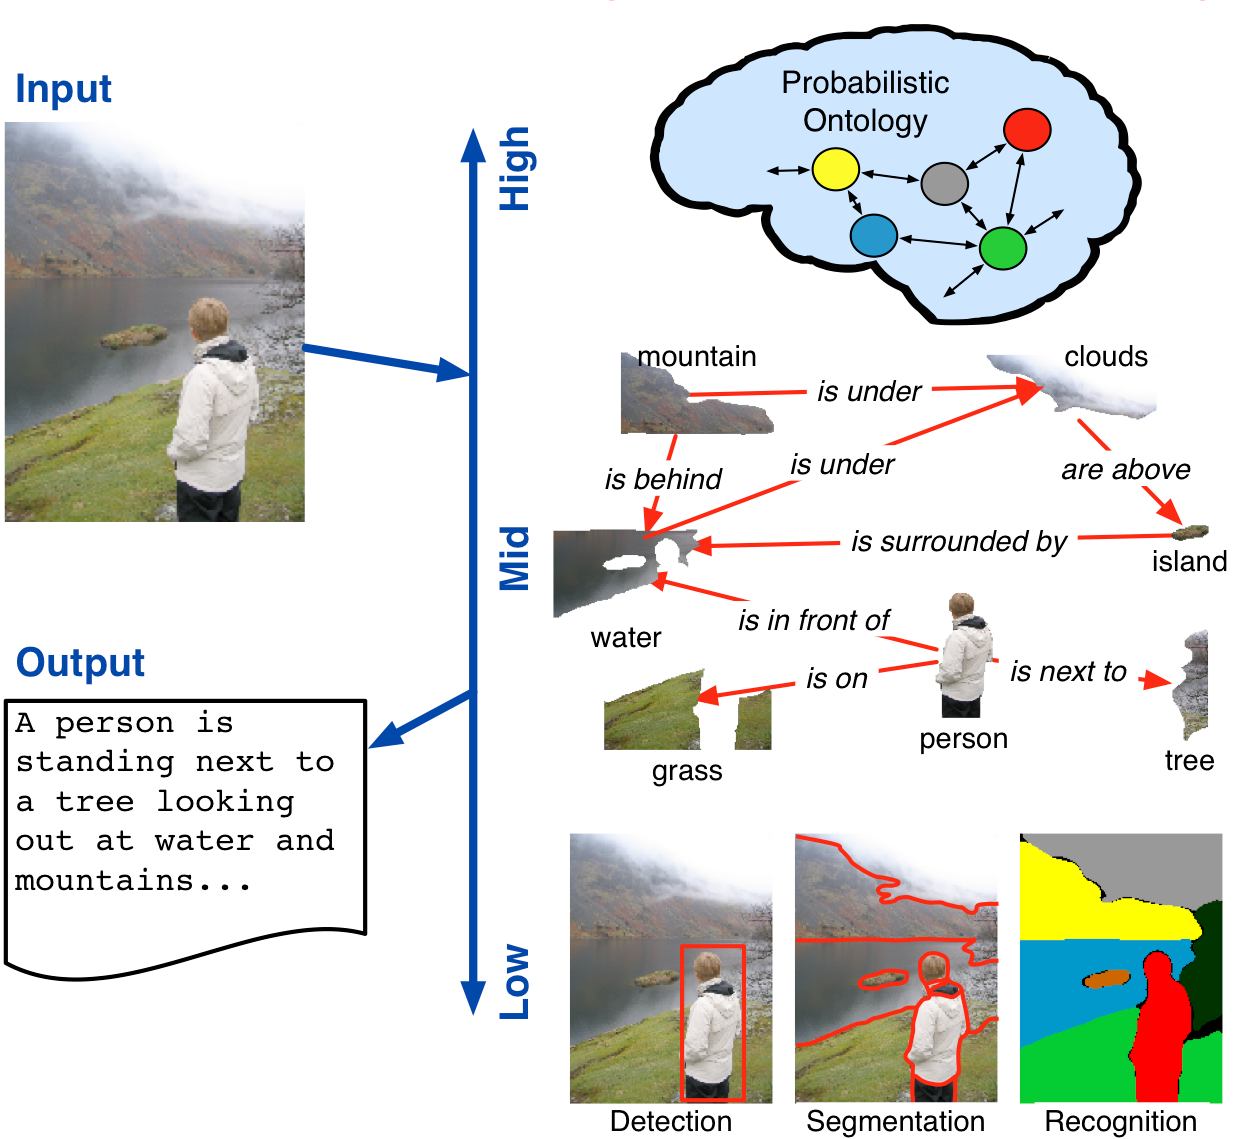
\includegraphics[width=\textwidth]{./img/motivation1.png} 
		\begin{scriptsize} \begin{center}
			\textbf{Generalized Image Understanding with Probabilistic Ontologies \footnotemark}
		\end{center} \end{scriptsize} 
    \end{subfigure}\hspace{1em}%
    \begin{subfigure}[c]{0.2\textwidth}
		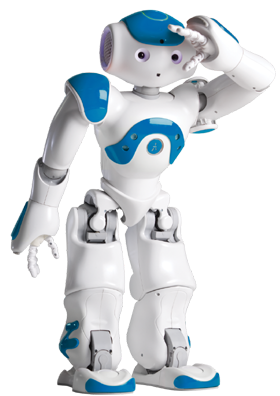
\includegraphics[width=\textwidth]{./img/motivation2.png} 
		\begin{scriptsize} \begin{center}
		 \textbf{Alderbaran robot Nao \footnotemark}
		\end{center} \end{scriptsize} 
    \end{subfigure}%
    

\end{figure}

\footnotetext[1]{\tiny{~\url{http://blog.zanox.com/en/zanox/2014/07/29/already-benefiting-power-online-videos/}}}
\footnotetext[2]{\tiny{~\url{http://www.cse.buffalo.edu/~jcorso/r/career}}}
\footnotetext[3]{\tiny{~\url{https://www.aldebaran.com/en/humanoid-robot/nao-robot}}}

\end{frame}

\begin{frame}{\textbf{Objective}}
	\begin{columns}
		\begin{column}{0.55\textwidth}
		\begin{varblock}[\textwidth]{Problem}
			To detect and identify events in a given video segment.
		\end{varblock}
		\begin{varblock}[\textwidth]{Challenges}
			\begin{itemize}
				\item Geometric and photometric variances
				\item Cluttered	 background 
				\item Complex camera motion
			\end{itemize}
		\end{varblock}
		\begin{varblock}[\textwidth]{Applications}
			\begin{itemize}
				\item Real time event recognition
				\item Automated video annotation
			\end{itemize}
		\end{varblock}
		\end{column}
		\begin{column}{0.38\textwidth}
		\begin{figure}
			\centering
			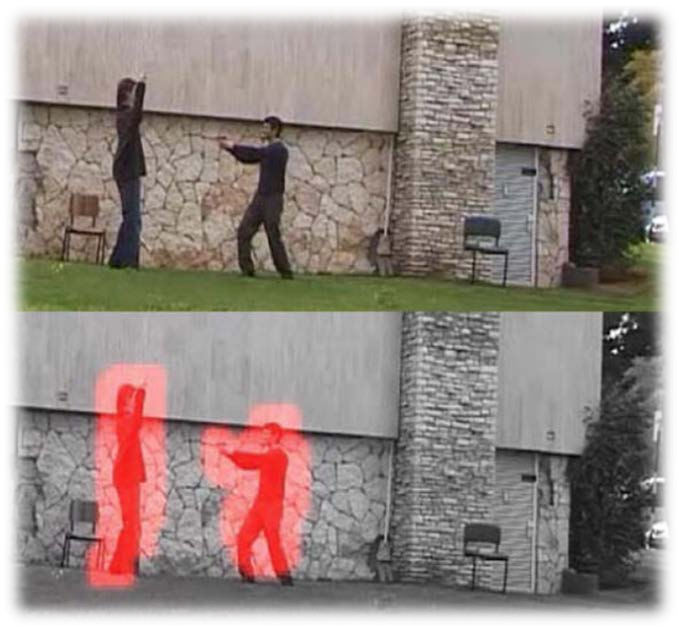
\includegraphics[width=\textwidth]{./img/example.png} 
			 \begin{scriptsize} \begin{center}
		 	\textbf{UCSD Anomaly Detection Dataset \footnotemark}
			\end{center} \end{scriptsize} 	
		\end{figure}
		\end{column}
	\end{columns}
\footnotetext[4]{\tiny{\url{http://www.svcl.ucsd.edu/projects/anomaly}}}
\end{frame}


\begin{frame}{\textbf{Proposed Framework}}
\begin{columns}
	\begin{column}{0.6\textwidth}
	\begin{figure}
	\begin{framed}
		\centering
		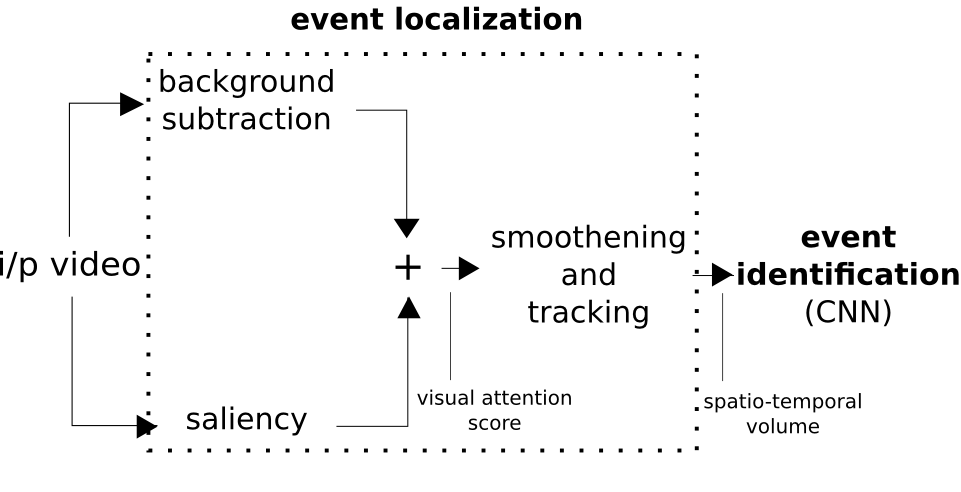
\includegraphics[width=\textwidth]{./img/outline.png}
	\end{framed}
		\caption{Proposed framework for video event recognition.}
	\end{figure}
	\end{column}
	\begin{column}{0.3\textwidth}
		\begin{varblock}[\textwidth]{Event localization}
			\textbf{Why do we need?} Most of the videos are weakly labeled they don't have spatial and temporal segmentation.
		\end{varblock}
		\begin{varblock}[\textwidth]{Event identification}
			Predict event label for given Spatio temporal volume (STV).
		\end{varblock}
	\end{column}
\end{columns}
\end{frame}

\begin{frame}{\textbf{Related work}}
\begin{columns}
	\begin{column}{0.45\textwidth}
		\begin{varblock}[\textwidth]{Spatial Event Localization}
			\begin{itemize}							
				\item Selective search of object of intereset after hierarchical segmentation\footnotemark.
				\item Merge super-voxel segments based on motion features\footnotemark.
			\end{itemize}
		\end{varblock}
	\end{column}
	\begin{column}{0.45\textwidth}
		\begin{varblock}[\textwidth]{Event Identification}
		 Generally such problems are tackled in following manner: 
			\begin{itemize}
				\item local feature extraction
				\item feature aggregation
				\item classifier (such as SVM) to distinguish
			\end{itemize}
		\end{varblock}
	\end{column}
\end{columns}	
\footnotetext[5]{\tiny{Lampert, Christoph H., Matthew B. Blaschko, and Thomas Hofmann. "Beyond sliding windows: Object localization by efficient subwindow search." Computer Vision and Pattern Recognition, 2008. CVPR 2008. IEEE Conference on. IEEE, 2008.}}
\footnotetext[6]{\tiny{Jain, Mihir, Jan van Gemert, Hervé Jégou, Patrick Bouthemy, and Cees GM Snoek. "Action localization with tubelets from motion." In Computer Vision and Pattern Recognition (CVPR), 2014 IEEE Conference on, pp. 740-747. IEEE, 2014.}}
\end{frame}
